\documentclass[aspectratio=169]{beamer}

\usetheme[font=noto,summary]{UiO}

\usepackage[utf8]{inputenc}
\usepackage{babel}

\usepackage[backend=biber,style=authoryear,maxcitenames=2]{biblatex}
\addbibresource{Library.bib}

\usepackage{graphicx}
\usepackage{booktabs}
\usepackage{hyperref}
\usepackage{tikz}
\usetikzlibrary{positioning, shapes, arrows.meta}

\title[Protocol Racing]{Protocol Racing}
\subtitle{Is it really an advancement?}
\author[Joar Heimonen]{Joar Heimonen}
\date{\today}
\uioemail{contact@joar.me}

\begin{document}

\uiofrontpage[dept={}, image={image.png}, inverted]

\begin{frame}{Agenda}
  \tableofcontents
\end{frame}

\section{A bit of history}
\begin{frame}{IPv4}
  \begin{itemize}
    \item \textbf{RFC 791} – \emph{Internet Protocol}
    \item Written for DARPA in 1981 (before the IETF existed)
    \item Designed to interconnect different packet-switched networks (ARPANET, SATNET, university nets)
    \item Created under the assumption that every device would have its own globally unique, routable address
    \item 32-bit address space — \(2^{32} = 4{,}294{,}967{,}296\) possible addresses
    \item Sounds like a lot\ldots\ until you remember that there are 8 billion people alive
  \end{itemize}
\end{frame}

\begin{frame}{The problem with IPv4}
  \centering
  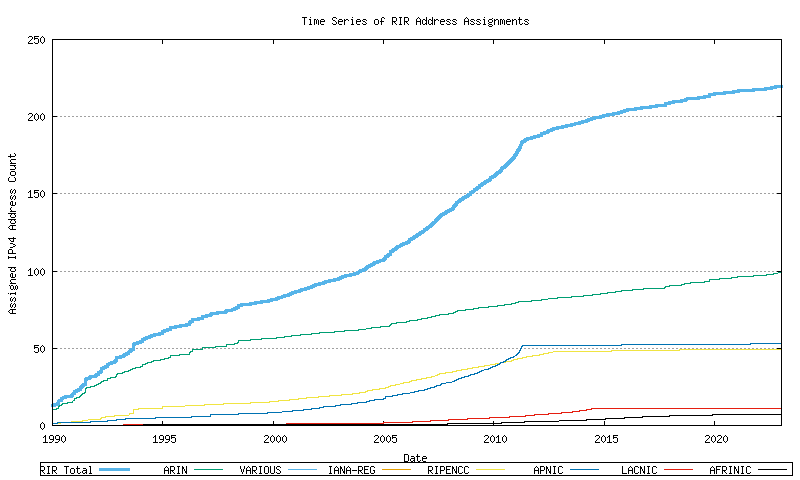
\includegraphics[width=0.8\textwidth]{fig09.png}
  \\
  {\tiny Source: \parencite{IPv4AddressReport}}
\end{frame}

\begin{frame}{Timeline of stopgap measures}
\centering
\small
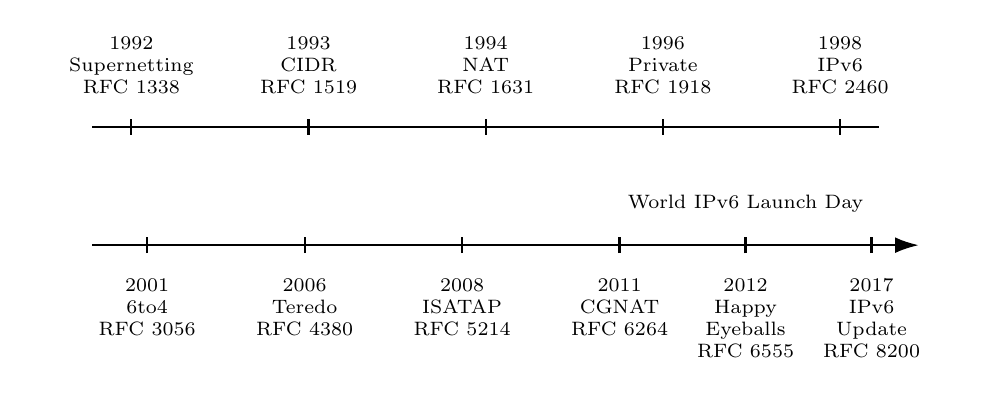
\begin{tikzpicture}[
    x=1cm, y=1cm,
    every node/.style={align=center,font=\scriptsize},
    >=Latex
]
    \def\upperY{0.8}
    \def\lowerY{-0.7}

    \draw[thick] (0, \upperY) -- (10, \upperY);
    \draw[thick, -{Latex[length=3mm,width=2mm]}] (0, \lowerY) -- (10.5, \lowerY)
        node[right, font=\scriptsize, xshift=2mm] {};

    \foreach \xu/\txt in {
        0.5/{1992\\Supernetting\\RFC 1338},
        2.75/{1993\\CIDR\\RFC 1519},
        5.0/{1994\\NAT\\RFC 1631},
        7.25/{1996\\Private\\RFC 1918},
        9.5/{1998\\IPv6\\RFC 2460}
    }{
        \draw[thick] (\xu, \upperY-0.1) -- (\xu, \upperY+0.1);
        \node[above=3mm, text width=2.4cm] at (\xu, \upperY) {\txt};
    }

    \foreach \xl/\txt in {
        0.7/{2001\\6to4\\RFC 3056},
        2.7/{2006\\Teredo\\RFC 4380},
        4.7/{2008\\ISATAP\\RFC 5214},
        6.7/{2011\\CGNAT\\RFC 6264},
        8.3/{2012\\Happy\\Eyeballs\\RFC 6555},
        9.9/{2017\\IPv6\\Update\\RFC 8200}
    }{
        \draw[thick] (\xl, \lowerY-0.1) -- (\xl, \lowerY+0.1);
        \node[below=3mm, text width=2.4cm] at (\xl, \lowerY) {\txt};
    }

    \def\ipv6LaunchX{8.3} % align with 2012 Happy Eyeballs; adjust slightly if needed
    \draw[thick] (\ipv6LaunchX, \lowerY-0.1) -- (\ipv6LaunchX, \lowerY+0.1);
    \node[above=3mm, text width=3cm] at (\ipv6LaunchX, \lowerY) {World IPv6 Launch Day};
\end{tikzpicture}

\vspace{0.4cm}
\footnotesize
\textit{Timeline of stopgap measures from Supernetting (aggregation strategy) to IPv6 'v2'}
\end{frame}

\section{Main}
\begin{frame}{Key Idea}
  \begin{block}{Takeaway}
    Keep each slide focused on one idea.
  \end{block}
\end{frame}

\section{Wrap-up}
\begin{frame}
  \centering
  \vfill
  {\usebeamerfont{title}\usebeamercolor[fg]{title}\LARGE Questions?}
  \vfill
\end{frame}

\begin{frame}[allowframebreaks]{References}
  \printbibliography
\end{frame}
\end{document}
